\section{Conclusion} \label{sec:conclusion}
The Synapse-191 project started as a fun challenge: could we build a full computer, from scratch, that speaks Brainf*ck as its native language? Not because it’s practical—because it’s interesting. Bit by bit, the design grew into a complete system: a microcoded CPU with a clean Harvard-like architecture, a two-phase clock, a working toolchain, and a surprisingly advanced I/O module. Somewhere along the way, the breadboards turned into a small city of logic chips, wires, and LEDs that somehow cooperate well enough to run real programs.

That’s not to say it’s perfect. In fact, it never has been fully stable. Especially the cheaper breadboards, some of which are still part of the system, proved to be have unreliable power rails. Bad connections to power or ground often lead to hard-to-debug problems. Still, the system works well enough to demonstrate every part of the design, and it’s a small miracle that it does so as reliably as it does.

If there’s ever a “next step,” it would be to take everything learned from this messy forest of jump wires and translate it onto a proper PCB. That would eliminate most of the grounding and signal integrity issues and turn this hand-built prototype into a stable, portable machine.

But even as it stands, the BFCPU has been a fantastic experiment—one that turned abstract ideas about microarchitecture, control logic, and timing into something you can literally touch. It’s a reminder that sometimes the best way to understand how computers work isn’t to simulate them, but to build one with your own hands—and then spend months trying to figure out why it occasionally forgets what “ground” means.

\mbox{}
\vfill
\begin{figure}[H]
  \centering
  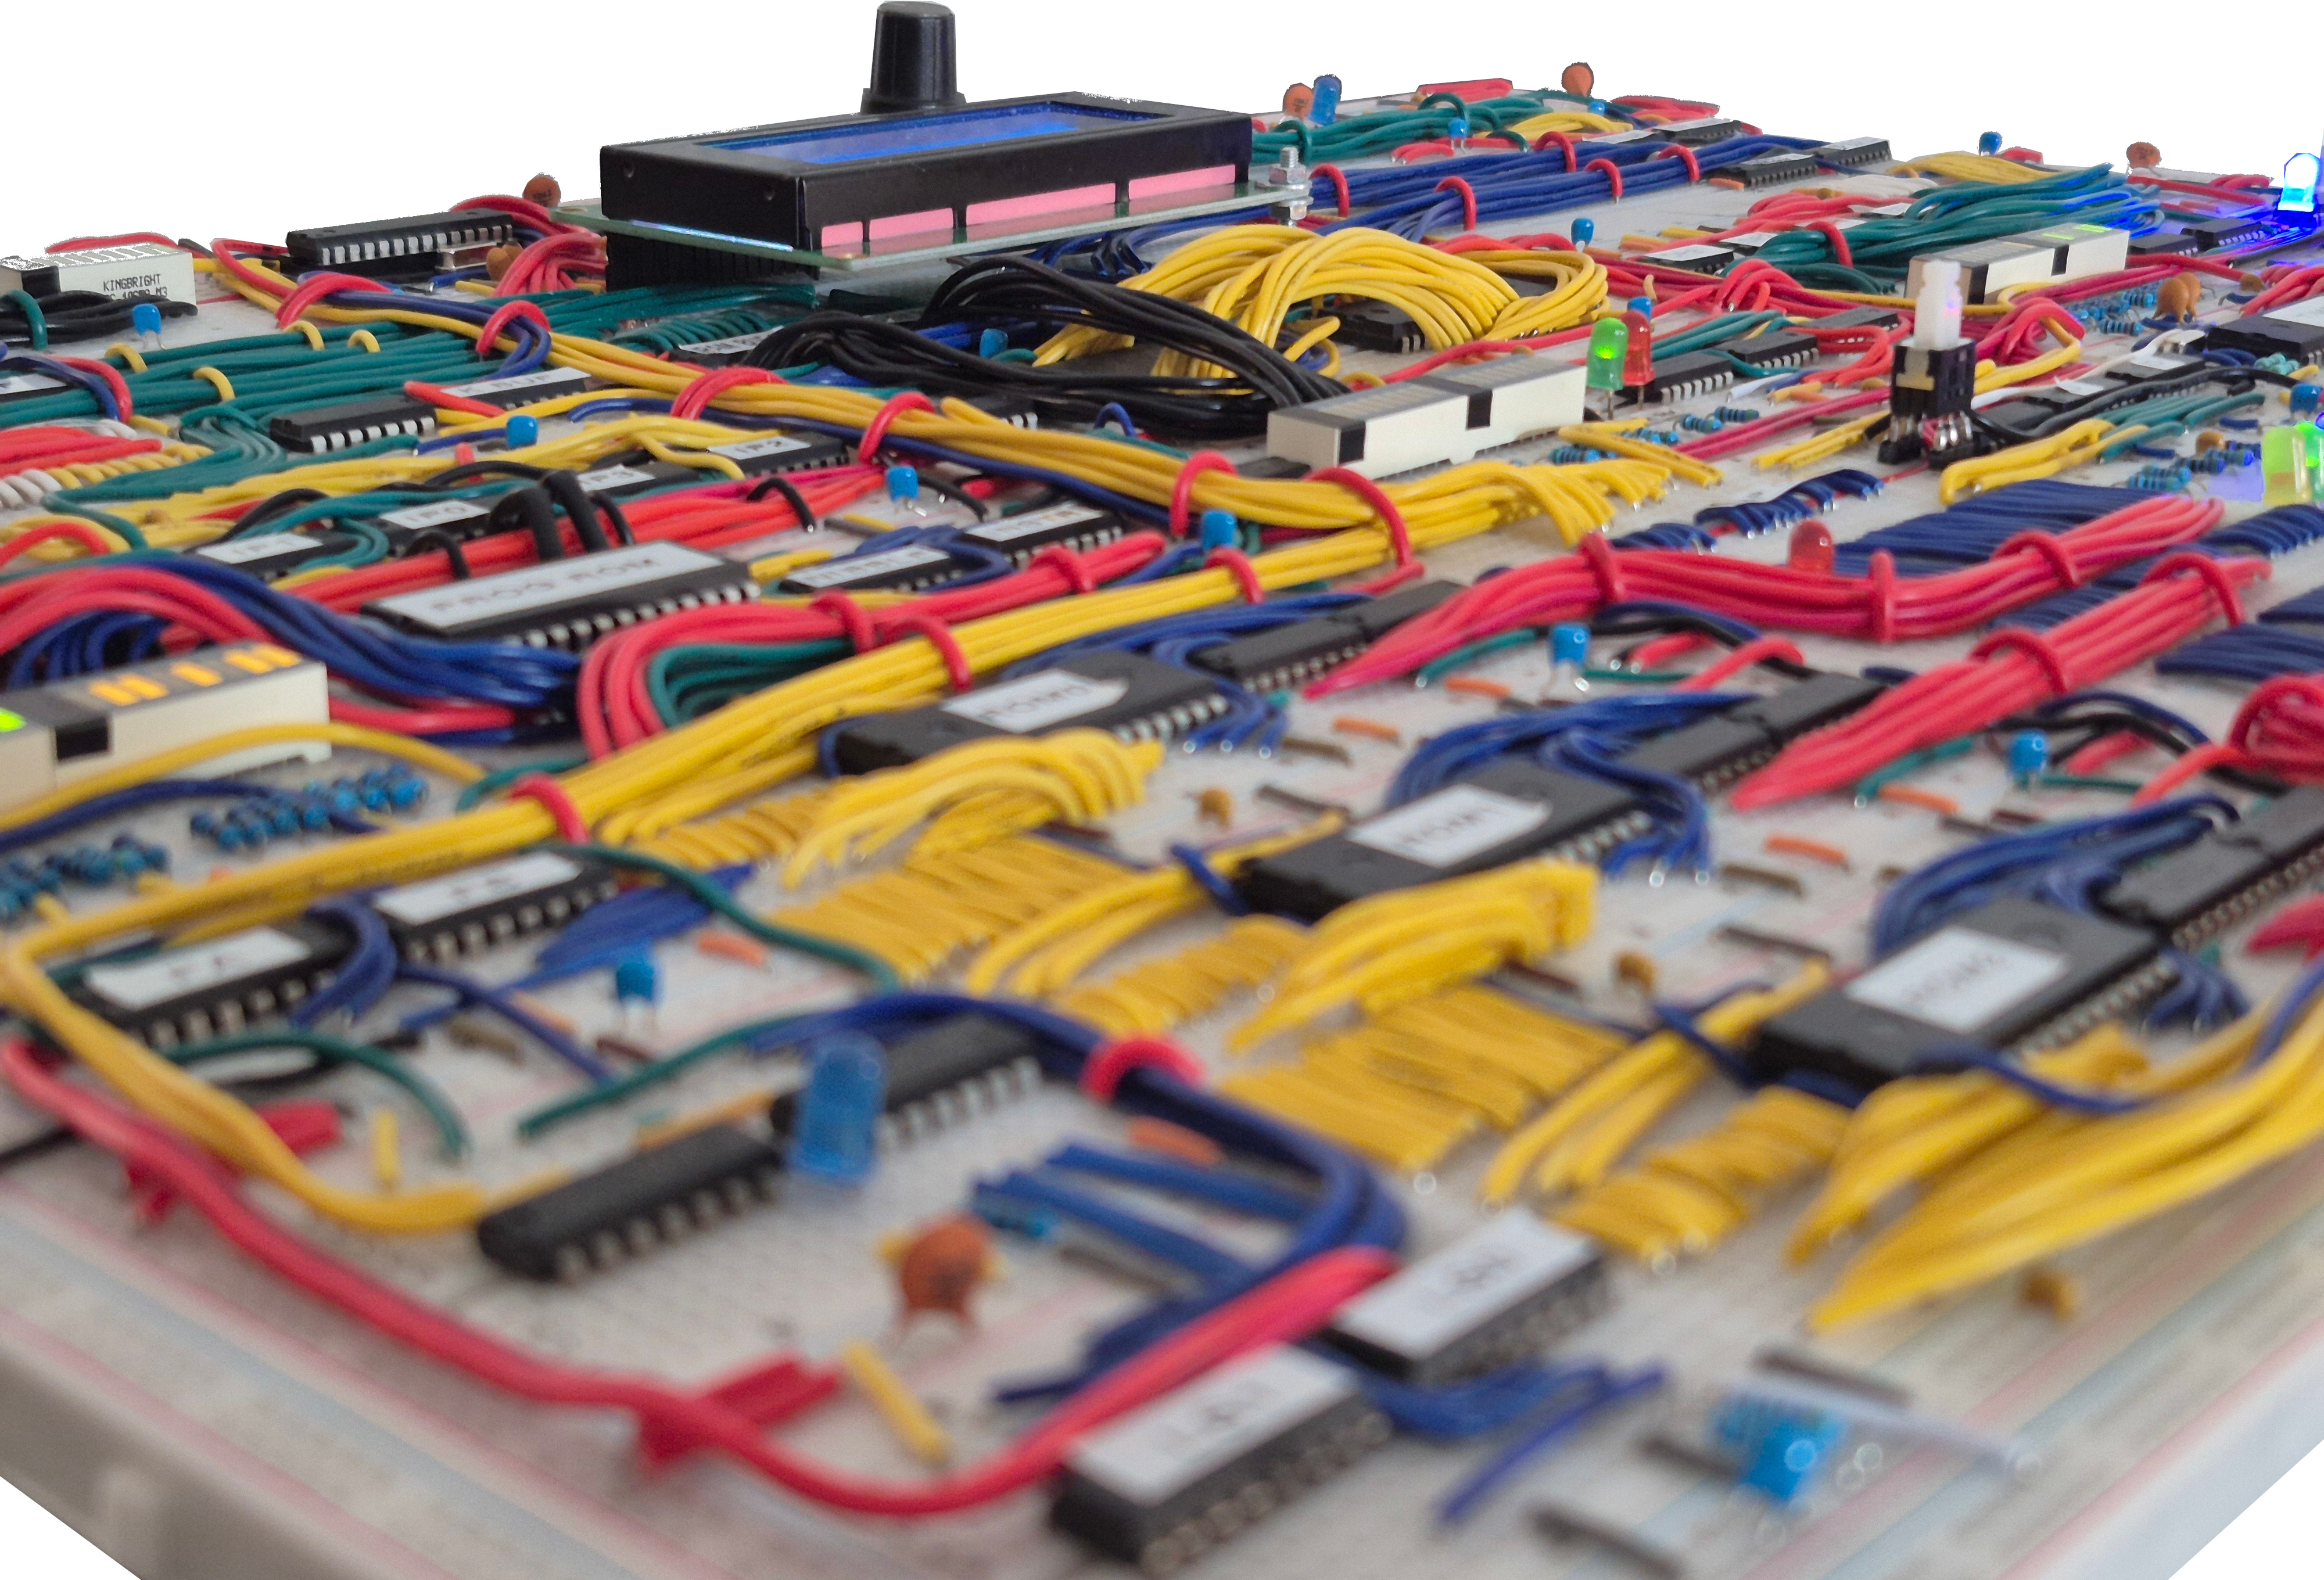
\includegraphics[width=\textwidth]{img/final_img}
\end{figure}


